\section*{Ethics}

\prob{4} Which ethics principle described in the Belmont
Report best describes informed consent? \\ (Select the best answer.)\\
\correctanswercircle{Respect for Autonomy} \\
\answercircle{Justice}\\
\answercircle{Beneficience}\\
\answercircle{Respect for Public Policy}\\
\answercircle{None of the above}
\eprob


\begin{center}
\framebox[0.9\linewidth]{
\parbox{0.8\linewidth}{
    {\bf Case Study:}
    hiQ Labs, a data analytics company, used web scraping to gather publicly
    accessible data from LinkedIn profiles to analyze employee turnover
    trends. LinkedIn objected, claiming this scraping violated its terms of
    service and potentially compromised user privacy. They argued that users
    consented to LinkedIn's terms, which restrict data usage, and that
    scraping compromised user expectations of privacy. LinkedIn also applied
    technical barriers to prevent hiQ from accessing its data, which hiQ
    circumvented.

    hiQ argued that the data it accessed was publicly available, and LinkedIn
    had no grounds to restrict access under the Computer Fraud and Abuse Act
    (CFAA), which typically protects against unauthorized access to private
    data. hiQ contended that restricting access to this data hampered
    competition and limited the public’s ability to analyze openly accessible
    information on the internet.
}
    }
\end{center}

\prob{4} Use the principle of {\em beneficience} to present an
argument {\bf in
favor} of the experiment.\\
\answerbox{2.5}{
hiQ Labs’ use of publicly accessible LinkedIn data could be justified by the
principle of beneficence, as it aims to generate insights that could benefit
employees and employers, for example by predicting metrics such as turnover
trends. This data analysis could potentially lead to better workplace policies
and improved job satisfaction from these insights.
}
\eprob

\pagebreak
\prob{4} Use the principle of {\em beneficience} to present an
argument {\bf against}
the experiment.\\
\answerbox{2.5}{
From a beneficence perspective, hiQ Labs’ actions could be argued against if
the scraping activity compromises individual privacy or leads to unintended
negative consequences, such as privacy violations or misuse of personal data.
This harm to LinkedIn users’ expectations of privacy might outweigh the
potential benefits to companies or researchers from analyzing turnover trends.
}
\eprob


\prob{4} 
Edward Snowden, a former NSA contractor, released classified information in
2013 revealing that the NSA was conducting extensive, indiscriminate
surveillance on American citizens and foreign nationals. This surveillance
included monitoring phone calls, internet activity, and communications data
without individuals' knowledge or consent, raising significant concerns about
privacy and government overreach.

Snowden believed that individuals had a right to know how their personal
information was being used. Which ethical principle does this belief best
align with?\\
\correctanswercircle{Respect for Autonomy} \\
\answercircle{Justice}\\
\answercircle{Beneficience}\\
\answercircle{Respect for Public Policy}\\
\answercircle{None of the above}
\eprob

\prob{2}
Institutional Review Board (IRB) approval of a research study implies that the
study is ethical.\\
\yesnono
\eprob

\section*{Denial of Service Attacks}

\prob{2}  
Identify and circle the part of the
Internet infrastructure responsible for sending reflected DNS traffic to the
target. \\ \vspace*{-0.1in}
\begin{center}
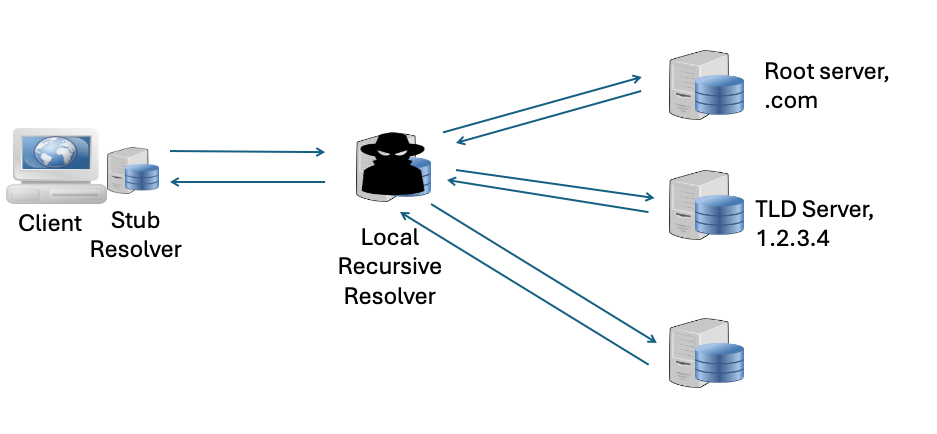
\includegraphics[width=0.8\textwidth]{dns2.png}  
\end{center}
\eprob

\prob{4}  Which of the following is an example of amplification? (Select all
that apply.)\\
\correctanswercircle{A small DNS query results in a DNS response that is
redirected to a target IP address.} \\
\answercircle{A large number of packets is sent to a single IP address.} \\
\correctanswercircle{A ``ping'' to a broadcast address generates reply
messages sent to a target IP address.} \\
\answercircle{A large number of packets is sent to a single port.} \\
\eprob


\prob{2} Which of the following are characteristics of denial of service
attacks? (Select all that apply.)\\
\correctanswercircle{They are often launched from multiple sources.} \\
\correctanswercircle{The traffic they generate can be difficult to distinguish
from legitimate traffic.} \\
\correctanswercircle{They often involve ``amplification'' techniques.} \\
\answercircle{They always involve exhaustion of network bandwidth.} \\
\eprob

\section*{Public Key Infrastructure}

\prob{4}  In the assignment, you visited a website that used a self-signed
certificate. Which of the following statements is true?\\
\correctanswercircle{Many browsers will issue warnings when visiting a website with self-signed certificate.}\\
\answercircle{A self-signed certificate is as secure as a certificate signed by a certificate authority.}\\
\correctanswercircle{Traffic can be encrypted with a self-signed certificate
if the server uses a secure protocol like HTTPS.}\\
\correctanswercircle{The server can be impersonated by an attacker if it uses a
self-signed certificate.}\\
\eprob

\prob{4}  
Which of the following statements correctly describes the role of a
Certificate Authority (CA) in Public Key Infrastructure (PKI)? (Select all
that apply.)\\
\correctanswercircle{A CA issues digital certificates that verify the
ownership of public keys used in secure communications.}\\
\answercircle{A CA encrypts all communication between clients and servers in a
PKI.}\\
\correctanswercircle{A CA is responsible for verifying the identity of
entities before issuing certificates.}\\
\answercircle{A CA stores the private keys of all clients in a PKI.}\\
\correctanswercircle{If a CA's private key is compromised, attackers could
potentially impersonate any entity certified by that CA.}\\
\eprob

\newpage
\prob{4}  
Describe where Root Certificate Authorities (Root CAs) are typically stored in
a client’s environment.\\ 
\answerbox{2}{
    Root Certificate Authorities (Root CAs) are typically stored in the
    operating system’s trusted certificate store on a client’s device. This
    storage location allows the system and applications, such as web browsers,
    to reference these trusted Root CAs to verify the authenticity of digital
    certificates when establishing secure connections.
}
\eprob

\prob{2}
Which aspects of the infrastructure must users trust when using Public Key
Infrastructure (PKI)?\\
\correctanswercircle{The integrity of Root CAs.}\\
\correctanswercircle{The security of Root CAs' private keys.}\\
\correctanswercircle{The reliance on Certificate Authorities to properly
verify entities before issuing certificates.}\\
\answercircle{The security of the network over which the root CAs are transmitted.}\\
\eprob

\prob{3}
Suppose an attacker is able to install a "rogue" root CA on your machine. Which of the following
statements is true about the incident? (Select all that apply.)\\
\correctanswercircle{The attacker may be able to decrypt all past and future messages sent to the
server.}\\
\answercircle{Using the private key, an attacker can impersonate clients to the server.}\\
\correctanswercircle{Using the private key, an attacker can impersonate the server to clients.}\\
\answercircle{The server can prevent against eavesdropping attacks by revoking its certificate.}\\
\answercircle{All of the above}
\eprob


\section*{Web Security}

\prob{4}  
Given the following URL to a JavaScript file that dynamically displays
messages on the web page: \url{https://example.com/displayMessage?message=}
This script accepts a URL parameter `message` to display a custom message on
the page.  
Modify the URL to attempt injecting JavaScript that turns all of the
text on the page red.  Precise/correct syntax is not required, and pseudocode
is fine. Show the general approach. \\
\answerbox{2.5}{
To inject JavaScript that turns all of the text on the page red, one might
modify the URL parameter `message` to include a script tag that applies inline
CSS styling to change the font color. For instance, the URL might look like: 
\url{https://example.com/displayMessage?message=<script>document.body.style.color='red';</script>}
}
\eprob

\newpage
\prob{3}  
Which of the following best describes the concept of "origin" in the context
of the Same-Origin Policy? (Select one.)\\
\correctanswercircle{The combination of protocol, hostname, and port of a
URL.}\\
\answercircle{The domain name of the website only.}\\
\answercircle{The IP address of the server serving the webpage.}\\
\answercircle{Only the protocol (e.g., HTTP or HTTPS) of the webpage.}\\
\eprob



\prob{4}  
Which of the following actions can help prevent Cross-Site Scripting (XSS)
attacks? (Select all that apply.)\\
\correctanswercircle{Sanitizing user input to remove or encode potentially
harmful characters.}\\
\correctanswercircle{Validating and restricting the types of inputs allowed
(e.g., only allowing alphanumeric characters where possible).}\\
\answercircle{Allowing users to input and execute JavaScript code in their
profiles.}\\
\correctanswercircle{Escaping output in HTML templates to prevent injected
scripts from running.}\\
\answercircle{Disabling cookies on the client’s browser.}\\
\eprob


\section*{DNS Security and Privacy}

\prob{2} Provide an argument for why DNS-over-HTTPS, as implemented in today's
web browsers, might {\bf improve}
privacy and security for Internet users. \\
\answerbox{2.5}{
    DNS-over-HTTPS (DoH) improves privacy by encrypting DNS queries, which
    prevents third parties, such as ISPs or local network operators, from
    viewing the domain names that a user is visiting. This encryption provides
    users with more control over their browsing privacy and helps protect
    against certain types of surveillance or data collection.
}
\eprob

\prob{2} Provide an argument for why DNS-over-HTTPS, as implemented in today's
web browsers, might {\bf degrade}
privacy and security for Internet users. \\
\answerbox{2.5}{
    DNS-over-HTTPS (DoH) might degrade privacy and security because it
    centralizes DNS queries to specific providers, which could lead to
    increased tracking by those providers. Additionally, if these centralized
    DoH providers are compromised, it could expose sensitive browsing
    information for numerous users at once.
}
\eprob

\prob{2}
When encrypted DNS is enabled in your browser, the operator of the local WiFi
network can no longer see the domain names that you are visiting.\\
\yesnoyes
\eprob

\section*{Privacy and Tracking}

\prob{4}  
Which of the following are commonly used techniques for web browser
fingerprinting? (Select all that apply.)\\
\correctanswercircle{Collecting information about the user's browser and
operating system settings, such as screen resolution and
language.}\\
\correctanswercircle{Using JavaScript to analyze hardware information, like
the number of CPU cores and available memory.}\\
\answercircle{Identifying users solely based on IP address.} \\
\correctanswercircle{Tracking installed browser plugins and fonts to create a
unique user profile.}\\
\answercircle{Requiring users to log in to verify their identity on each
visit.}\\
\eprob

\prob{4} If a user deletes cookies from a web browser after every visit to a
webpage, does it prevent the website from tracking users across visits?\\
\yesnono
\eprob

\prob{4}
Why or why not? \\
\answerbox{2.5}{
    No, deleting cookies alone does not prevent tracking across visits. Websites
    can use other tracking techniques, such as browser fingerprinting, which
    collect information about the user's device and browser configuration to
    create a unique identifier. This identifier remains even after cookies are
    deleted, allowing websites to recognize users across visits.
}
\eprob

\section*{Feedback}
\vspace*{-0.1in}
\prob{1}
Interest (1=Boring!; 10=Amazing!):
\shortanswerbox{0.5}{5}
Difficulty (1=Too easy; 10=Too hard):
\shortanswerbox{0.5}{5}
\eprob
\prob{1}
1. One thing you like. 2. One suggestion for improvement:

\answerbox{0.75}{More free food.}
\eprob

